% Primeiro Exame

%1 Architecture Influence Cycle - REUSED
\newcommand{\qArchitectureInfluenceCycle}{
\begin{ClosedQuestion}
  The software architecture of a system

    \optionA{Depends mostly on the system's functional requirements.}
    \optionB{Depends more on the architect's experience than on anything
    else.}
    \optionC{Should not depend on the skills of the developing team.}
    \optionD{Is driven by a trade-off among the stakeholders needs.}
 \putOptions 
\end{ClosedQuestion}
}


%2 Pragmatic Architect
\newcommand{\qTechoGeeks}{
\begin{ClosedQuestion}
    Frank Buschmann, \emph{Introducing the Pragmatic Architect}, defines the \emph{techno-geeks} architects. This kind of architect
    
    \optionA{May be responsible for the Featuritis problems of architectures.}
    \optionB{May be responsible for the Performitis problems of architectures.}
    \optionC{Is focused on creating common generalizations of several systems.}
    \optionD{Is focused on the details of the architecture.}
 \putOptions
\end{ClosedQuestion}
}


%3 Featuritis Performitis Flexibilities
\newcommand{\qFeaturitisOrderPad}{
\begin{ClosedQuestion}
    Frank Buschmann states that:
        
    \begin{quote}
        Featuritis is the tendency to trade functional coverage for quality - the more functions the earlier they're delivered, the better.
    \end{quote}
    
    In the OrderPad system the architect regretted not getting performance tests going earlier. The OrderPad system

    \optionA{Suffered from featuritis, because the architect decided to delay the difficult parts for latter in the development.}
    \optionB{Did not suffer from featuritis.}
    \optionC{Suffered from some level of featuritis, but it allowed to have a pilot from which the team learned.}
    \optionD{Suffered from featuritis, but it had no impact on the final development.}
 \putOptions 
\end{ClosedQuestion}
}

%4 Architecture Definition - REUSED
\newcommand{\qArchitectureDefinition}{
\begin{ClosedQuestion}
  The software architecture of a system

  \optionA{Is a high-level view of the system with the purpose of
  understanding what are the system's goals and features.}
  \optionB{Is composed of things such as code units, runtime elements,
  hardware, and people, together with the relationships among them.}
  \optionC{Is a set of guidelines that the developing team should
  follow in the development of the system.}
  \optionD{Is a set of diagrams that show the runtime elements of the
  system and their relationships.}
 \putOptions 
\end{ClosedQuestion}
}

%5 Module vs Component - REUSED
\newcommand{\qModuleComponent}{
\begin{ClosedQuestion}
  Which of the following phrases best describe the relationship
  between modules and components?

  \optionA{A module may contain code from different components.}
  \optionB{A component may execute code from different modules.}
  \optionC{A module may execute code from different components.}
  \optionD{A component may contain code from different modules.}
 \putOptions 
\end{ClosedQuestion}
}

%6 Scenarios and Tactics
\newcommand{\qScenario}{
\begin{ClosedQuestion}
    Consider the following scenario
    
    \begin{quote}
        Our vehicle information system send our current location to the traffic monitoring system. The traffic monitoring system combines our location with other information, overlays this information on a Google Map, and broadcasts it. Our location information is correctly included with a probability of 99.99\%.
    \end{quote}
    
    \optionA{The current location is the source of the stimulus.}
    \optionB{The traffic monitoring system is the environment.}
    \optionC{The Google Map is the artefact.}
    \optionD{The location information is correctly included with a probability of 99.99\% is the response measure.}
 \putOptions
\end{ClosedQuestion}
}

%7 Availability
\newcommand{\qChecksum}{
\begin{ClosedQuestion}
    Checksum is a technic that it is often used in architectural design. It can be used as
        
    \optionA{A Condition Monitoring tactic for the Availability quality.}
    \optionB{An Encrypt Data tactic for the Security quality.}
    \optionC{A Verify Message Integrity tactic to React to Attacks for the Security quality.}
    \optionD{An Exception Prevention tactic to Prevent Faults for the Availability quality.}
 \putOptions
\end{ClosedQuestion}
}

%8 Security
\newcommand{\qAttack}{
\begin{ClosedQuestion}
    An attack is
        
    \optionA{The source of stimulus for scenarios of the Availability quality.}
    \optionB{The stimulus for scenarios of the Availability quality.}
    \optionC{The stimulus for scenarios of the Security quality.}
    \optionD{The source of stimulus for scenarios of the Security quality.}
 \putOptions
\end{ClosedQuestion}
}

%9 SocialCal Scenarios and Tactics
\newcommand{\qSocialCalcTactics}{
\begin{ClosedQuestion}
    In the description of the SocialCalc case study can be read:
    
    \begin{quote}
        As the user scrolls the spreadsheet through our custom-drawn scroll bars, we dynamically update the innerHTML of the pre-drawn \textsc{<td>} elements. This means we don't need to create or destroy any \textsc{<tr>} or \textsc{<td>} elements in many common cases, which greatly speeds up response time.
    \end{quote} 
    
    This corresponds to the application of

    \optionA{Manage sampling rate tactic.}
    \optionB{Increase resource efficiency tactic.}
    \optionC{Introduce concurrency tactic.}
    \optionD{Schedule resources tactic.}
 \putOptions
\end{ClosedQuestion}
}

%10 Thounsand Parsec Scenarios and Tactics
\newcommand{\qThousandParsecTactics}{
\begin{ClosedQuestion}
    In the description of the Thousand Parsec case study can be read:
    
    \begin{quote}
        A ruleset designer thus has the ability to create new object types or store additional information in the existing object types as required by the ruleset, allowing for virtually unlimited extensibility in terms of the available physical objects in the game.
    \end{quote} 
    
    This excerpt can be represented as a modifiability scenario where

    \optionA{The source of stimulus is the ruleset.}
    \optionB{The ruleset designer is the stimulus.}
    \optionC{The environment is design time.}
    \optionD{The response is defer binding.}
 \putOptions
\end{ClosedQuestion}
}

%11 Git and GitHub Scenarios and Tactics
\newcommand{\qGitTactics}{
\begin{ClosedQuestion}
    In the description of the Git case study can be read:
    
    \begin{quote}
        Git tackles the storage space problem by packing objects in a compressed format, using an index file which points to offsets to locate specific objects in the corresponding packed file.
    \end{quote}
    
    The tactic addressed in this fragments is:
    
    \optionA{Schedule resources.}
    \optionB{Condition monitoring.}
    \optionC{Reduce overhead.}
    \optionD{Increase resource efficiency.}
 \putOptions
\end{ClosedQuestion}
}


%12 Designing-an-Architecture - REUSED
\newcommand{\qDesigningArchitecture}{
\begin{ClosedQuestion}
  The architectural significant requirements are important in the process of creating
  the software architecture for a system because they define
 
  \optionA{The most important requirements (both functional and
  qualities) that the system must achieve.}
  \optionB{How the components manage the communication between the
  remaining elements in the system.}
  \optionC{The stakeholders that drive the development of the system.}
  \optionD{The tactics that satisfy the most important requirements for
  the system.}
 \putOptions 
\end{ClosedQuestion}
}

%13 Module Viewtype - REUSED
\newcommand{\qDecompositionGeneralization}{
\begin{ClosedQuestion}
  Consider that a chess game should
  provide an automatic and intelligent chess player, and that to
  implement that player we will use some of the many chess engines
  already available in the market.  Moreover, the system should allow
  the user to choose which engine to use for each new game.  Given
  these requirements, which of the architectural styles from the
  module viewtype are best suited to satisfy them?
 
  \optionA{The Decomposition style.}
  \optionB{The Decomposition and Uses styles.}
  \optionC{The Layered style.}
  \optionD{The Generalization and Decomposition styles.}
 \putOptions 
\end{ClosedQuestion}
}

%14 Uses and Generalization architectural styles - REUSED
\newcommand{\qUsesStyle}{
\begin{ClosedQuestion}
  To achieve a faster time-to-market, software companies are
  increasingly using a strategy of incremental releases of their
  software, where each new release has a set of new features.  Which
  architectural style is better to analyse whether the system's
  software architecture is adequate for the planned incremental
  releases?
 
  \optionA{The Decomposition style.}
  \optionB{The Deployment style.}
  \optionC{The Uses style.}
  \optionD{The Work-assignment style.}
 \putOptions 
\end{ClosedQuestion}
}

%15 Layered, Aspects and Data Model - REUSED
\newcommand{\qLayered}{
\begin{ClosedQuestion}
  Assume that one of the requirements for a graphical chess game is
  that it should be able to run both in Microsoft's Windows and
  Apple's Mac OS X operating systems.  A good solution for this system
  would:

  \optionA{Create a decomposition where there is a module corresponding
  to the Windows OS and another one for the Mac OS X, each one
  responsible for containing the OS-specific code.}
  \optionB{Use a classic 3-layer architecture with the following
  layers, from top to bottom: Presentation, Domain Logic, and Data
  Access.}
  \optionC{Use an aspect-oriented architecture, where an aspect is used to generate a graphical interface.}
  \optionD{Use two deployment views, each one allocating different
  components to different machines with different operating systems.}
 \putOptions 
\end{ClosedQuestion}
}

%16 Component and Connector
\newcommand{\qInterfaceDelegation}{
\begin{ClosedQuestion}
    Consider the concept of interface delegation 
        
    \optionA{It corresponds to a particular case of a specialization in a generalization view.}
    \optionB{It represents a relation between a connector's role and a port of one of its internal components.}
    \optionC{It represents a relation between a component's port and a port of one of its internal components.}
    \optionD{It represent a relation between a component's port and a connector's role.}
 \putOptions
\end{ClosedQuestion}
}


%17 Repository and Client-Server - REUSED
\newcommand{\qRepository}{
\begin{ClosedQuestion}
  A requirement for a chess game is that it keeps a table with the best scores obtained in the game.
  Naturally, this information should be kept between two different
  executions of the system.  Assuming that the game is a web-based application, then

  \optionA{We have to use a Repository component-and-connector style.}
  \optionB{It is not necessary to use a ``Data Access'' layer because the information is simple.}
  \optionC{We must identify a module for writing the scores in a
  Decomposition style.}
  \optionD{We may assign the responsibility of writing the scores to
  another module that already has other responsibilities.}
 \putOptions 
\end{ClosedQuestion}
}

%18 Tiers, Dynamic reconfiguration, Peer-to-peer, Publish-subscribe - REUSED
\newcommand{\qPeerToPeer}{
\begin{ClosedQuestion}
  An email client such as Mozilla's Thunderbird or Microsoft's Outlook
  allows a user both to read the emails that were sent to him and to
  send new emails to other people.  To do that, the email client
  connects to other components (one or more): some of these components
  keep the user's mailboxes with all the emails that were sent to him,
  whereas other components know how to forward the emails sent by the
  user to their final destinations (associated with a new set of destinations).  In either case, it is always the
  email client that makes a request to the other components, but
  whereas in the first case the email client receives all the
  information about the user's emails, in the second case only a
  success or failure error code is returned.  The architectural
  patterns that best describe the interactions between the components from the client to the final destinations

  \optionA{Client-server in both cases.}
  \optionB{Client-server in the first case and Peer-to-peer in the second.}
  \optionC{Peer-to-peer in both cases.}
  \optionD{Peer-to-peer in the first case and Client-Server in the second.}
 \putOptions 
\end{ClosedQuestion}
}

%19 SOA, Pipes-and-Filters - REUSED
\newcommand{\qPipesFilters}{
\begin{ClosedQuestion}
    Consider that you intend to develop a system where it is necessary to change the emails received by the server (for instance, to remove potential virus or URLs for phishing sites). The goal is that each email is processed by this system before it is sent to other servers or it is stored locally. Additionally, the system should be easily modified to support new kinds of transformations. Which style is more suitable to satisfy these requirements? 

    \optionA{Peer-to-Peer.}
    \optionB{Pipe-and-Filter.}
    \optionC{Client-Server.}
    \optionD{Publish-Subscribe.}
 \putOptions
\end{ClosedQuestion}
}

%20 Allocation viewtype
\newcommand{\qInstallView}{
\begin{ClosedQuestion}
  Consider a system that will require a significative configuration effort during deployment, because it provides several variations of the same functionalities and it is necessary to choose which functionalities better fit in each case. The most helpful architectural view for this situation is
 
  \optionA{Work assignment view.}
  \optionB{Install view.}
  \optionC{Implementation view.}
  \optionD{Deployment view.}
 \putOptions
\end{ClosedQuestion}
}

%21 ThousandParsec views
\newcommand{\qThounsandParsecView}{
\begin{ClosedQuestion}
    Consider the architectural views for the ThousandParsec system. In the case description can be read:
    
    \begin{quote}
        The Requirements function verifies that each component added to the design conforms to the rules of other previously added components.
    \end{quote}
    
    The following diagram depicts a fragment of a proposal for the decomposition view of the system.
    
    \begin{center}
    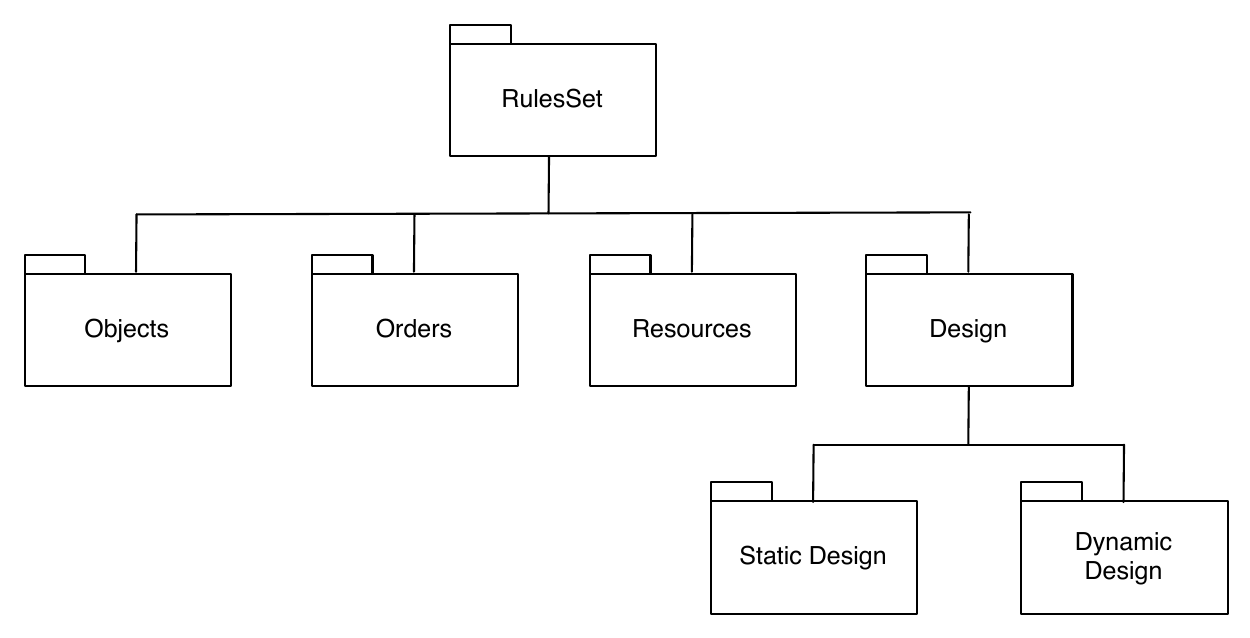
\includegraphics[width=100mm]{x-ThousandParsec-ruleset}
  \end{center}

    \optionA{The Requirements function is part of the Design module.}
    \optionB{The Requirements function is not part of the RulesSet module.}
    \optionC{The Requirements function is part of the Objects module.}
    \optionD{The Requirements function is part of the Dynamic Design module.}
 \putOptions
\end{ClosedQuestion}
}

%22 SocialCalc Views
\newcommand{\qSocialCalcView}{
\begin{ClosedQuestion}
    Consider the architectural views for the SocialCalc system. In the case description can be read:
    
    \begin{quote}
        The save format is in standard MIME multipart/mixed format, consisting of four text/plain; charset=UTF-8 parts, each part containing newline-delimited text with colon-delimited data fields. The parts are...
        
        This format is designed to be human-readable, as well as being relatively easy to generate programmatically. This makes it possible for Drupal's Sheetnode plugin to use PHP to convert between this format and other popular spreadsheet formats, such as Excel (.xls) and OpenDocument (.ods).
    \end{quote}
    
    From the above excerpt can be inferred the need to have
    
    \optionA{A component-and-connector view using a shared-data style.}
    \optionB{A data model view.}
    \optionC{A service-oriented architecture view.}
    \optionD{A data model view and a component-and-connector view using a shared-data style.}
 \putOptions
\end{ClosedQuestion}
}

%23 Git and GitHub Views
\newcommand{\qGitViews}{
\begin{ClosedQuestion}
    The architectural style that best represents the runtime execution of a system Git installed for a small group of developers is
            
    \optionA{Peer-to-peer style.}
    \optionB{Pipe-and-Filter style.}
    \optionC{Shared-data style.}
    \optionD{Publish-subscribe style.}
 \putOptions
\end{ClosedQuestion}
}

%24 The architecture of the OrderPad
\newcommand{\qOrderPad}{
\begin{ClosedQuestion}
  In the OrderPad system they have decided to use a Row Data Gateway data access pattern because
 
  \optionA{The team did not know the FenixFramework.}
  \optionB{The domain only needs CRUD (Create, Read, Update, and Delete) operations.}
  \optionC{A domain layer is absent from the architecture.}
  \optionD{Most of the information is stored in the client.}
 \putOptions
\end{ClosedQuestion}
}

%25-28 EtherCalc - 4
\newcommand{\qEtherCalcAllocation}{
\begin{ClosedQuestion}
  Consider the architectural views of EtherCalc system. In the case study description can be read
  
  \begin{quote}
      The Socialtext platform has both behind-the-firewall and on-the-cloud deployment options, imposing unique constraints on EtherCalc's resource and performance requirements.
  \end{quote} 
 
  \optionA{It is necessary to design two deployment views, one for each deployment option.}
  \optionB{It is necessary to design a single deployment view that contains all the variation, because only the hardware capabilities change.}
  \optionC{Two different component-and-connector views are necessary to represent the same runtime behavior of the system.}
  \optionD{The deployment options have a large impact on the work assignment view.}
 \putOptions
\end{ClosedQuestion}
}

\newcommand{\qEtherCalcRedundancy}{
\begin{ClosedQuestion}
  In EtherCalc initial prototype clients send their local commands and snapshots to the server, which result on redundant information on the server about the state of the spreadsheet. This redundancy is an application of
 
  \optionA{Passive redundancy for availability, because it is possible to recover from the commands log.}
  \optionB{Undo tactic for usability, because the server can undo the snapshot.}
  \optionC{Increase resource efficiency tactic for performance, because it reduces the need of upfront calculus/computation on new clients.}
  \optionD{Multiple copies of data tactic for performance, clients do not have to execute the commands.}
 \putOptions
\end{ClosedQuestion}
}

\newcommand{\qEtherCalcSnapshotPerformance}{
\begin{ClosedQuestion}
  In EtherCalc initial prototype clients send their local commands, cursor movements and snapshots to the server.
 
  \optionA{The server propagates them to all the clients.}
  \optionB{The server propagates local commands and cursor movements to the clients, and keeps the snapshots for the initialization of new clients.}
  \optionC{The server only propagates local commands to the clients and keeps cursor movements in a log and the snapshots in a repository.}
  \optionD{The server propagates the snapshots and the cursor movements to the clients and store the local commands for the initialization of new clients.}
 \putOptions
\end{ClosedQuestion}
}


\newcommand{\qEtherCalcModifiabilityTestability}{
\begin{ClosedQuestion}
  In the EtherCalc case description can be read
 
  \begin{quote}
      The in-browser SocialCalc engine is written in JavaScript. We considered translating that logic into Perl, but that would have carried the steep cost of maintaining two code bases. 
  \end{quote} 
  
  The excerpt is referring to a quality of
 
  \optionA{Testability.}
  \optionB{Modifiability.}
  \optionC{Testability and Modifiability.}
  \optionD{Performance.}
 \putOptions
\end{ClosedQuestion}
}


%29-30 Domain Logic and Access Patterns

%29 - REUSED
\newcommand{\qServiceLayer}{
\begin{ClosedQuestion}
  The Service Layer pattern is typically used in conjunction with
 
  \optionA{The Transaction Script pattern to help demarcate the
  business transactions.}
  \optionB{The Domain Model pattern to reduce the interface of the
  Domain Logic layer to a controlled set.}
  \optionC{The Data Access layer to be able to access the data that it
  needs in each service.}
  \optionD{The Table Module pattern to hide the details of the table
  structure for the Presentation layer.}
 \putOptions
\end{ClosedQuestion}
}

%30 - REUSED
\newcommand{\qActiveRecord}{
\begin{ClosedQuestion}
  The Active Record pattern is best used when we are also using
 
  \optionA{The Transaction Script pattern.}
  \optionB{The Table Module pattern.}
  \optionC{The Domain Model pattern.}
  \optionD{The Service Layer pattern.}
 \putOptions
\end{ClosedQuestion}
}

% Segundo Exame

%1 Architecture Influence Cycle - REUSED
\newcommand{\qArchitectureKnowledge}{
\begin{ClosedQuestion}
  Assuming that you were asked to document the software architecture
  of an existing (and already developed) system, the best thing for
  you to do would be

  \optionA{To analyse the source code of the system to see how it is built}
  \optionB{To analyse the system's functional requirements to see what
  is the system supposed to do}
  \optionC{To analyse the implemented set of features to see what is it
  that the system actually does}
  \optionD{To talk with the people that developed the system to know
  what they did and why they did it}
 \putOptions
\end{ClosedQuestion}
}

%2 Pragmatic Architect
\newcommand{\qArchitectureEvolution}{
\begin{ClosedQuestion}
  Ralph Johnson says that
  
  \begin{quote}
      Architecture is the decisions that you wish you could get right early in a project.
  \end{quote}
  
  This sentence reflects the fact that

  \optionA{The architecture of a system cannot change}
  \optionB{The main goal of an architect is to identify the quality attributes of system}
  \optionC{Architecture is the design that gets harder to change as development progresses}
  \optionD{The main goal of an architect is to design a detailed structure of the system that supports most of the requirements}
 \putOptions
\end{ClosedQuestion}
}

%3 Featuritis Performitis Flexibilities
\newcommand{\qPerformitis}{
\begin{ClosedQuestion}
    Marquardt characterizes performitis as:
    
    \begin{quote}
        Each part of the system is directly influenced by local performance tuning measures. There is no global performance strategy, or it ignores other qualities of the system such as testability and maintainability.
    \end{quote}
    
    This means that

  \optionA{It is not a good idea to consider performance when designing the architecture of the system}
  \optionB{The performance of a system only depends on the global performance strategies} 
  \optionC{Testability and maintainability always conflict with performance} 
  \optionD{None of the above}
 \putOptions
\end{ClosedQuestion}
}


%4 Architecture Definition - REUSED
\newcommand{\qArchitecturalViews}{
\begin{ClosedQuestion}
    The software architecture of a system is usually represented through several views because we need to

  \optionA{Represent different architectural qualities and they may not be all represented in a single view}
  \optionB{Have a view for each stakeholder} 
  \optionC{Have at least a view for each viewtype} 
  \optionD{Have a view for each group of interconnected components, and very often a system has several groups of interconnected components}
 \putOptions
\end{ClosedQuestion}
}

%5 Module vs Component
\newcommand{\qModueComponent}{
\begin{ClosedQuestion}
  On the web page of Memcached can be read:
  
  \begin{quote}
      ..., high-performance, distributed memory object caching system, generic in nature, but intended for use in speeding up dynamic web applications by alleviating database load.
  \end{quote}
  
  According to this information, Memcached is

  \optionA{A module}
  \optionB{A component}
  \optionC{Both, a module and a component}
  \optionD{An allocation element}
 \putOptions
\end{ClosedQuestion}
}

%6 Scenarios and Tactics - REUSED
\newcommand{\qConcreteScenario}{
\begin{ClosedQuestion}
  As part of the process of creating an architecture, we talked about
  a framework for capturing some of the requirements for a system.  In
  this context, \textbf{concrete scenarios} are used for

  \optionA{Describing what are the qualities that the system should possess}
  \optionB{Describing a set of steps that a user of the system must
  perform to accomplish some task}
  \optionC{Describing a use case for the system that makes clear what
  should be the system's responses to each of the user's inputs}
  \optionD{Describing the system's features by way of different
  usage scenarios for it, in which users play the role of actors}
 \putOptions
\end{ClosedQuestion}
}

%7 Availability
\newcommand{\qAvailabilityPingEchoHeartbeat}{
\begin{ClosedQuestion}
    Ping-and-echo and Heartbeat are two availability tactics to detect faults.

    \optionA{Ping-and-echo requires the availability monitor to know the addresses of the components it is monitoring}
    \optionB{Heartbeat requires the availability monitor to confirm the reception of the signal}
    \optionC{In Ping-and-echo the availability monitor should always send the same request}
    \optionD{In Heartbeat, the monitored components can change the message rate}
 \putOptions
\end{ClosedQuestion}
}

%8 Security - REUSE
\newcommand{\qSecurityDatabase}{
\begin{ClosedQuestion}
    Consider that when designing the architecture of a web application, the architect intends to guarantee of the confidentiality of persistent data in face of an attack from a system administrator.

    \optionA{It is not possible to achieve this requirement. A non-architectural solution is to be careful when hiring system administrators}
    \optionB{It is necessary to use the authenticate authors tactic to authenticate system administrators before they access to the database}
    \optionC{It is necessary to use the encrypt data tactic to encrypt the information with a password that is in a configuration file}
    \optionD{It is necessary to use the encrypt data tactic to encrypt the information on the client web browser, before it is send to the web server}
 \putOptions
\end{ClosedQuestion}
}

%9 SocialCal Scenarios and Tactics
\newcommand{\qSocialCalcTactic}{
\begin{ClosedQuestion}
    In the description of the SocialCalc case study can be read:
    
    \begin{quote}
        A simple improvement is for each client to broadcast its cursor position to other users, so everyone can see which cells are being worked on.
    \end{quote}
    
    This sentence describes a tactic for usability which is

    \optionA{Maintain task model}
    \optionB{Maintain user model}
    \optionC{Maintain system model}
    \optionD{Aggregate}
 \putOptions
\end{ClosedQuestion}
}

%10 Thounsand Parsec Scenarios and Tactics
\newcommand{\qThousandParsecScenario}{
\begin{ClosedQuestion}
    In the description of the ThousandParsec case study can be read:
    
    \begin{quote}
        The Thousand Parsec Component Language (TPCL) exists to allow clients to create designs locally without server interaction - allowing for instant feedback about the properties, makeup, and validity of the designs. 
    \end{quote}
    
    From this sentence can be written

    \optionA{A scenario for performance associated with a multiple copies of computation tactic}
    \optionB{A scenario for usability associated with a support system initiative tactic}
    \optionC{A scenario for performance associated with a limit event response tactic}
    \optionD{A scenario for usability associated with a support user initiative tactic}
 \putOptions
\end{ClosedQuestion}
}

%11 Git and GitHub Scenarios and Tactics
\newcommand{\qGitTactic}{
\begin{ClosedQuestion}
    In the description of GitHub case study can be read
    
    \begin{quote}
        Once the Smoke proxy has determined the user's route, it establishes a transparent proxy to the proper file server. We have four pairs of fileservers. Their names are fs1a, fs1b, ..., fs4a, fs4b. These are 8 core, 16GB RAM bare metal servers, each with six 300GB 15K RPM SAS drives arranged in RAID 10. At any given time one server in each pair is active and the other is waiting to take over should there be a fatal failure in the master. All repository data is constantly replicated from the master to the slave via DRBD.
    \end{quote}
    
    In this description we can find the application of tactics like 

  \optionA{Multiple copies of computation}
  \optionB{Active redundancy}
  \optionC{Increase resource efficiency}
  \optionD{All of the above}
 \putOptions
\end{ClosedQuestion}
}

%12 Designing-an-Architecture - REUSED
\newcommand{\qArchitecturallySignificantRequirements}{
\begin{ClosedQuestion}
  According to the attribute-driven design process, we should design
  the software architecture for a system based on a selected list of
  requirements, which are called the \textit{architecturally significant requirements}.
  These architecturally significant requirements should be sorted according to their
  importance for the system's stakeholders because
 
    \optionA{We should always satisfy in the first place the requirements
    of the more important stakeholders (such as the client)}
    \optionB{If no order was established among them, we would not know
    from where should we start the design process}
    \optionC{If one of the stakeholders complains that her requirement
    is not satisfied, we may explain to her that there were other more
    important requirements first}
    \optionD{When it is not possible to satisfy all of the requirements
    optimally, we should be aware of their relative importance so that
    we may find a solution that corresponds to a satisfactory trade-off}
 \putOptions
\end{ClosedQuestion}
}

%13 Module Viewtype
\newcommand{\qModuleTraceability}{
\begin{ClosedQuestion}
    Views of the module viewtype can be used to support requirements traceability analysis, determine how the functional requirements of a system are supported. This is represented by
    
    \optionA{Decomposition view}
    \optionB{Data model view}
    \optionC{Generalization view}
    \optionD{Layered view}
 \putOptions
\end{ClosedQuestion}
}


%14 Uses and Generalization architectural styles - REUSED
\newcommand{\qGeneralizationInterfaces}{
\begin{ClosedQuestion}
    You have to develop an application that collects news from different web sources and process that information to present a digest to the application users. The different sources provide similar information through different interfaces (APIs). Additionally, the new sources may change the interfaces, for instance to enhance their service. Which architectural style can be used to represent this requirements?
    
    \optionA{Peer-to-Peer to represent the communication between the components}
    \optionB{Client-Server to represent the request the application makes to the different new sources}
    \optionC{Generalisation to represent an abstraction common to all interfaces and keep API-specific details in child modules}
    \optionD{Layers to create a virtual machine that hides the internals of the application from its users interface code to allow the support of different user interfaces}
 \putOptions
\end{ClosedQuestion}
}

%15 Layered, Aspects and Data Model - REUSED
\newcommand{\qUsesIncremental}{
\begin{ClosedQuestion}
  When designing the architecture for a system the architect realises that most of the modules have bidirectional uses relationships. This has impact on

    \optionA{Performance because there is an overhead of communication between the modules.}
    \optionB{Install because most of the modules need to be assigned to the same executable file}
    \optionC{Development because it is not possible to do incremental development}
    \optionD{Availability because if a module fails the failure easily propagates to all the other modules}
 \putOptions
\end{ClosedQuestion}
}

%16 Component and Connector - REUSED
\newcommand{\qComponentAndConnnector}{
\begin{ClosedQuestion}
    The Java web servers, like Tomcat, use threads to process requests. For each request they create (or reuse) a thread to process it.
    To draw a architectural view that describes this behaviour we should use 
    
    \optionA{A Module viewtype view}
    \optionB{A Allocation viewtype view}
    \optionC{A Communicating processes view}
    \optionD{A Install view}
 \putOptions
\end{ClosedQuestion}
}

%17 Repository and Client-Server - REUSED
\newcommand{\qLoadBalancer}{
\begin{ClosedQuestion}
    To increase the availability of a web application it is possible to use a load-balancer between the clients and the servers that detects server failures and transparently redirects the requests to the servers that are functioning properly. To represent this architecture

    \optionA{It is enough to show the load-balancer between the web clients machines and the servers machines using a deployment view}
    \optionB{It is necessary to change the connector between the web clients and the web servers, in the component-and-connector view, to show the semantics that is provided by the load-balancer}
    \optionC{It is necessary to create a uses view to show how clients require the correct functioning of servers} 
    \optionD{It is necessary to change the component-and-connector view to show the communicating processes}
 \putOptions
\end{ClosedQuestion}
}

%18 Tiers, Dynamic reconfiguration, Peer-to-peer, Publish-subscribe - REUSED
\newcommand{\qThreeTiers}{
\begin{ClosedQuestion}
  One way to increase the performance of a 3-tier enterprise
  application (with the standard separation in the web client, web
  server, and database tiers) is to replicate the web server tier and
  to add a load-balancer between the web clients and the web servers.
  Unfortunately, for some enterprise applications that option is not
  enough (or does not work at all), because

    \optionA{They have many different use cases, corresponding to many
    distinct user interfaces}
    \optionB{They have to process very large amounts of data in each request}
    \optionC{They need to be able to process concurrent requests from
    the users}
    \optionD{They have a very complex domain logic that requires much
    processing power for answering each request}
 \putOptions
\end{ClosedQuestion}
}

%19 SOA, Pipes-and-Filters
\newcommand{\qPublishSubscribe}{
\begin{ClosedQuestion}
  Typically, Instant Messaging clients have a window to list the contacts of the user, and
  show in that window the status of each contact (whether it is available, unavailable, busy,
  etc). Given that the status of a contact may be changed at any time, and that the contact's
  status is given by the Instant Messaging application of that contact, which architectural
  style represents best the interaction pattern between these components?

    \optionA{The Shared Data style}
    \optionB{The Pipes-and-filters style}
    \optionC{The Publish-subscribe style}
    \optionD{The Client-Server style}
 \putOptions
\end{ClosedQuestion}
}

%20 Allocation viewtype - REUSED
\newcommand{\qDeploymentPerformance}{
\begin{ClosedQuestion}
  In the software architecture of a system, the Deployment view is
  best suited for

    \optionA{Analysing the performance of the system}
    \optionB{Planning incremental releases of the system}
    \optionC{Estimating the effort needed to implement the system}
    \optionD{Analysing the system's portability and reusability}
 \putOptions
\end{ClosedQuestion}
}

%21 ThousandParsec views
\newcommand{\qThousandParsecPersistence}{
\begin{ClosedQuestion}
  In the description of ThousandParsec case study can be read
  
  \begin{quote}
      The flagship server, \textsc{tpserver-cpp}, provides an abstract persistence interface and a modular plugin system to allow for various database back ends. 
  \end{quote}
  
    This above sentence can be diagrammatically represented using
      
    \optionA{A generalisation architectural style}
    \optionB{An aspects architectural style}
    \optionC{A data model architectural style}
    \optionD{A shared-data architectural style}
 \putOptions
\end{ClosedQuestion}
}

%22 SocialCalc Views
\newcommand{\qSocialCalcBroadcastEvents}{
\begin{ClosedQuestion}
  Consider the (partial) component-and-connector view for the \textsc{:SpreasdSheet} component of the SocialCalc system
  
    \begin{center}
    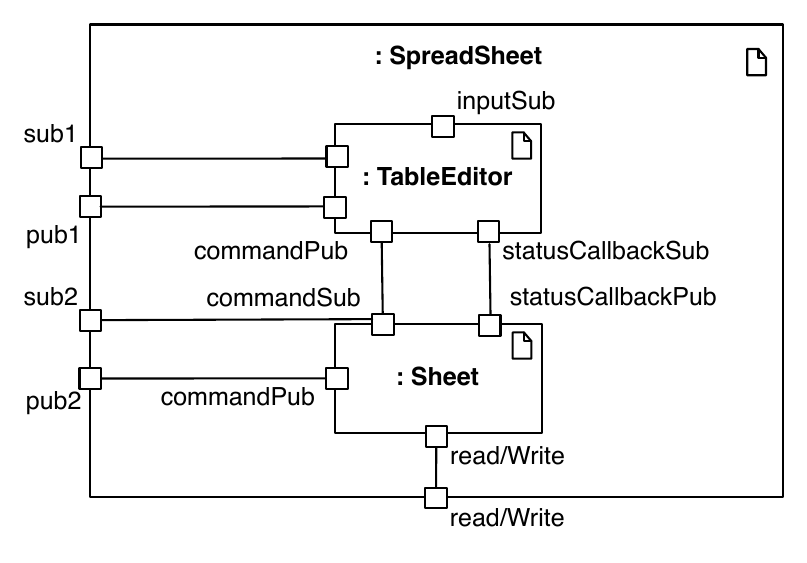
\includegraphics[width=70mm]{x-SocialCalc-spreadsheet-component}
  \end{center}
    
    \begin{flushleft}
        The \textsc{sub1} port
    \end{flushleft}

    \optionA{Subscribes to the same kind of events that the \textsc{sub2} port}
    \optionB{Subscribes to the same kind of events that the \textsc{inputSub} port}
    \optionC{Subscribes to cursor position events}
    \optionD{It is unnecessary in the diagram because the \textsc{:TableEditor} can use port \textsc{sub2} through the \textsc{:Sheet} component}
 \putOptions
\end{ClosedQuestion}
}

%23 Git and GitHub Views
\newcommand{\qGitHubViews}{
\begin{ClosedQuestion}
    In the description of GitHub case study can be read
    
    \begin{quote}
        For requests to the main website, the load balancer ships your request off to one of the four frontend machines. Each of these is an 8 core, 16GB RAM bare metal server. Their names are fe1, ..., fe4. Nginx accepts the connection and sends it to a Unix domain socket upon which sixteen Unicorn worker processes are selecting. One of these workers grabs the request and runs the Rails code necessary to fulfill it.
    \end{quote}
    
    To represent the above description it is necessary to use    

  \optionA{The communicating processes architectural style}
  \optionB{The client-server architectural style}
  \optionC{The deployment architectural style}
  \optionD{All of the above}
 \putOptions
\end{ClosedQuestion}
}

%24 The architecture of the OrderPad
\newcommand{\qOrderPadTactics}{
\begin{ClosedQuestion}
    In the description of architecture of the OrderPad case study, it can be read that the updates the user does on the OrderPad when it is offline are not lost. This availability quality is achieved through a    

  \optionA{Ignore faulty behaviour tactic}
  \optionB{Ping-and-echo tactic}
  \optionC{Active redundancy tactic}
  \optionD{Retry tactic}
 \putOptions
\end{ClosedQuestion}
}

%25-28 EtherCalc - 4

\newcommand{\qEtherCalcPerformance}{
\begin{ClosedQuestion}
    In the description of EtherCalc case study can be read
    
    \begin{quote}
        Because all jsdom code runs in a single thread, subsequent REST API calls are blocked until the previous command's rendering completes. Under high concurrency, this queue eventually triggered a latent bug that ultimately resulted in server lock-up.
    \end{quote}    
    
    The above sentence is related to a quality for

  \optionA{Performance, because it describes what is the response to REST API calls}
  \optionB{Modifiability, because the jsdom code can not be reused by several threads}
  \optionC{Security, because it describes a "queue overflow" attack}
  \optionD{Interoperability, because the REST API allow the exchange of information with external applications}
 \putOptions
\end{ClosedQuestion}
}

\newcommand{\qEtherCalcTactic}{
\begin{ClosedQuestion}
    In the description of EtherCalc case study can be read
    
    \begin{quote}
        So, we removed jsdom from the RenderSheet function, re-implemented a minimal DOM in 20 lines of LiveScript for HTML export, then ran the profiler again. Much better! We have improved throughput by a factor of 4, HTML exporting is 20 times faster, and the lock-up problem is gone.
    \end{quote}    
    
    The above sentence describes a

  \optionA{Reduce overhead tactic}
  \optionB{Increase resource efficiency tactic}
  \optionC{Increase resources tactic}
  \optionD{Testability tactic}
 \putOptions
\end{ClosedQuestion}
}

\newcommand{\qEtherCalcTestability}{
\begin{ClosedQuestion}
    In the description of EtherCalc case study can be read how the architect tried to increase the performance in a multi-core context
    
    \begin{quote}
    Is there a way to make use of all those spare CPUs in the multi-tenant server?

    For other Node.js services running on multi-core hosts, we utilized a pre-forking cluster server that creates a process for each CPU.
    
        However, while EtherCalc does support multi-server scaling with Redis, the interplay of Socket.io clustering with RedisStore in a single server would have massively complicated the logic, making debugging much more difficult.
    \end{quote}    
    
    This possible solution has impact on the

  \optionA{Overall costs, because of deployment}
  \optionB{Availability, because of the interprocess communication}
  \optionC{Testability, because of the logic complexity}
  \optionD{Performance, because there is not a significative improvement by using more CPUs}
 \putOptions
\end{ClosedQuestion}
}

\newcommand{\qEtherCalcViews}{
\begin{ClosedQuestion}
    In the description of EtherCalc case study can be read how the architect increased the performance in a multi-core context
    
    \begin{quote}
    Instead of pre-forking a fixed number of processes, we sought a way to create one background thread for each server-side spreadsheet, thereby distributing the work of command execution among all CPU cores.
    \end{quote}    
    
    Which is represented by the diagram
    \newline
    
    \begin{center}
    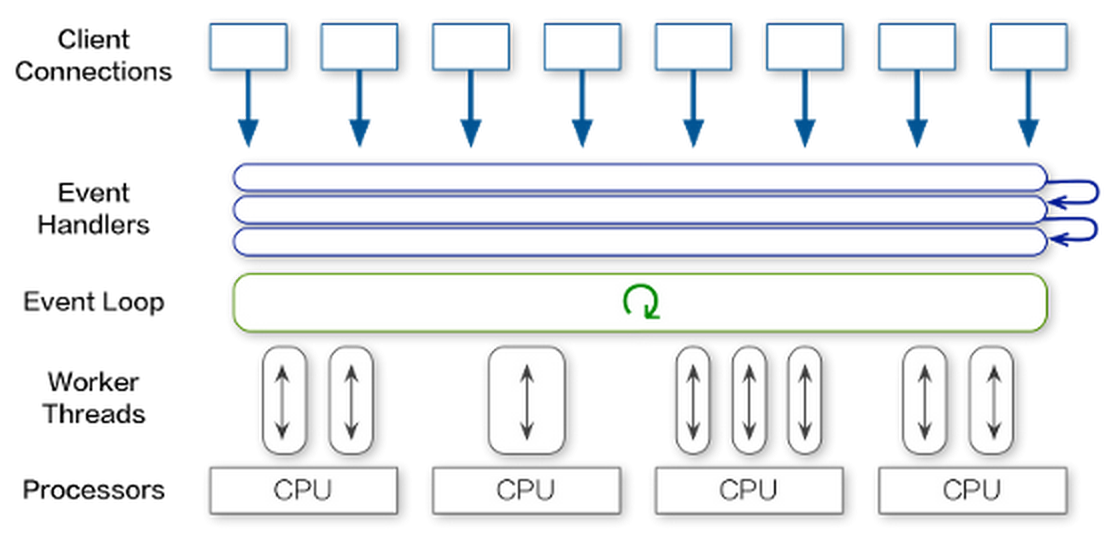
\includegraphics[width=120mm]{x-EtherCalc-multi-tenant}
  \end{center}
    
    \begin{flushleft}
        The above diagram, describing a server spreadsheet, can be represented using 
    \end{flushleft}

  \optionA{A publish-subscribe style}
  \optionB{A peer-to-peer style}
  \optionC{A client-server style}
  \optionD{A communication processes style}
 \putOptions
\end{ClosedQuestion}
}

%29-30 Domain Logic and Access Patterns - REUSED

\newcommand{\qTransactionScript}{
\begin{ClosedQuestion}
  Compared to the Transaction Script pattern, the Domain Logic pattern
  has a higher initial cost of adoption.  That is, it is harder to
  start with the Domain Logic pattern than with the Transaction Script
  pattern.  The reason for this is that the Domain Logic pattern

  \optionA{Requires a more skilled team, because the object-oriented
  paradigm is more complex than the procedural paradigm}
  \optionB{Is typically used with more complex data access code}
  \optionC{Requires that we write more code when we have only a
  couple of simple use cases}
  \optionD{All of the above}
 \putOptions
\end{ClosedQuestion}
}

\newcommand{\qActiveRecordRuby}{
\begin{ClosedQuestion}
  Ruby on Rails is a popular full-stack framework for building web
  applications.  One of the elements of this framework is the
  \textbf{model}, which is described in the Rails documentation in the
  following way:
  \begin{quote}
    A model represents the information (data) of the application and
    the rules to manipulate that data. In the case of Rails, models
    are primarily used for managing the rules of interaction with a
    corresponding database table. In most cases, one table in your
    database will correspond to one model in your application. The
    bulk of your application's business logic will be concentrated in
    the models.
  \end{quote}
  Given this description, the Rails' model is best described as an
  instance of
 
  \optionA{The Service Layer pattern}
  \optionB{The Active Record pattern}
  \optionC{The Transaction Script pattern}
  \optionD{The Data Mapper pattern}
 \putOptions
\end{ClosedQuestion}
}